\documentclass{article}
\usepackage{graphicx}
\usepackage{subfig}
\usepackage{amsmath}
\begin{document}
\section{Related Works} 
\subsection{Preliminaries}
\subsubsection{Motivation: Data Integrity Threat Model for Processor-Memory Architecture}
In the scenario of processor-memory architecture, data integrity refers to maintaining the data on the transmission outside the chip and stored on off-chip memory untampered. If the data stored on off-chip memory , or some external data injected to the system S, we can say that the data integrity of S is attacked. If the system S can not examine the tampered data or injected data, the attack is assumed to be successful. According to our knowledge, there are two aspects of attacks on data integrity:
\begin{enumerate}
	\item Introducing new content: The content of data in the system is modified, or data construct by the attacker is inserted to the system.
	\item Replacing data with valid copy: The data D in transmission or on the memory is replace with the following two types of copy: A copy of D at an old time point or a copy of other data from different memory address.
\end{enumerate}

\subsubsection{Protection of Integrity: Theoretical Models}
The goal of integrity protection can be defined as the capability to examine whether the data to read by processor has been tampered. According to our knowledge, there are three common types of cryptographic primitives aiming to protect the data integrity of a system, which are cryptographic hash function, Message Authentication Code(MAC) scheme and block-level Added Redundancy Explicit Authentication (AREA). These theoretical models for integrity protection is also called Authentication Primitives(AP) in some research works.

\paragraph{Cryptographic Hash Functions}
Hash is a short message block computed by hash function with data block D as input.
When processor writes a data block to a memory address, the data block D is sent to Hash function and a Hash value H1 is computed and stored on the chip. The hash value H is stored on chip following the order of data block on the memory. The message stored on the memory from chip is data block D alone.
When the processor wants to read a data block D from memory, D is sent to hash function and an hash value H2 is computed. If H1 is identical to H2, then the data block D is assumed to be untampered and read by processor.

Figure 3-a expresses functionality of hash function in integrity protection.
If the integrity of a processor-memory system is protected by hash function, the possible attacks are:
\begin{enumerate}
	\item Modify the content of a data block
	\item Insert new data
	\item Replace the content of a data block with a copy of data from other address
\end{enumerate}
If using hash function to protect integrity, the three attacks in the above list can be defended if the hash function behave like an theoretical random function, which means for any input data block D, its hash value H is randomly assigned.

\paragraph{Message Authentication Code(MAC) Schemes}
\begin{figure}[htbp]
\centering
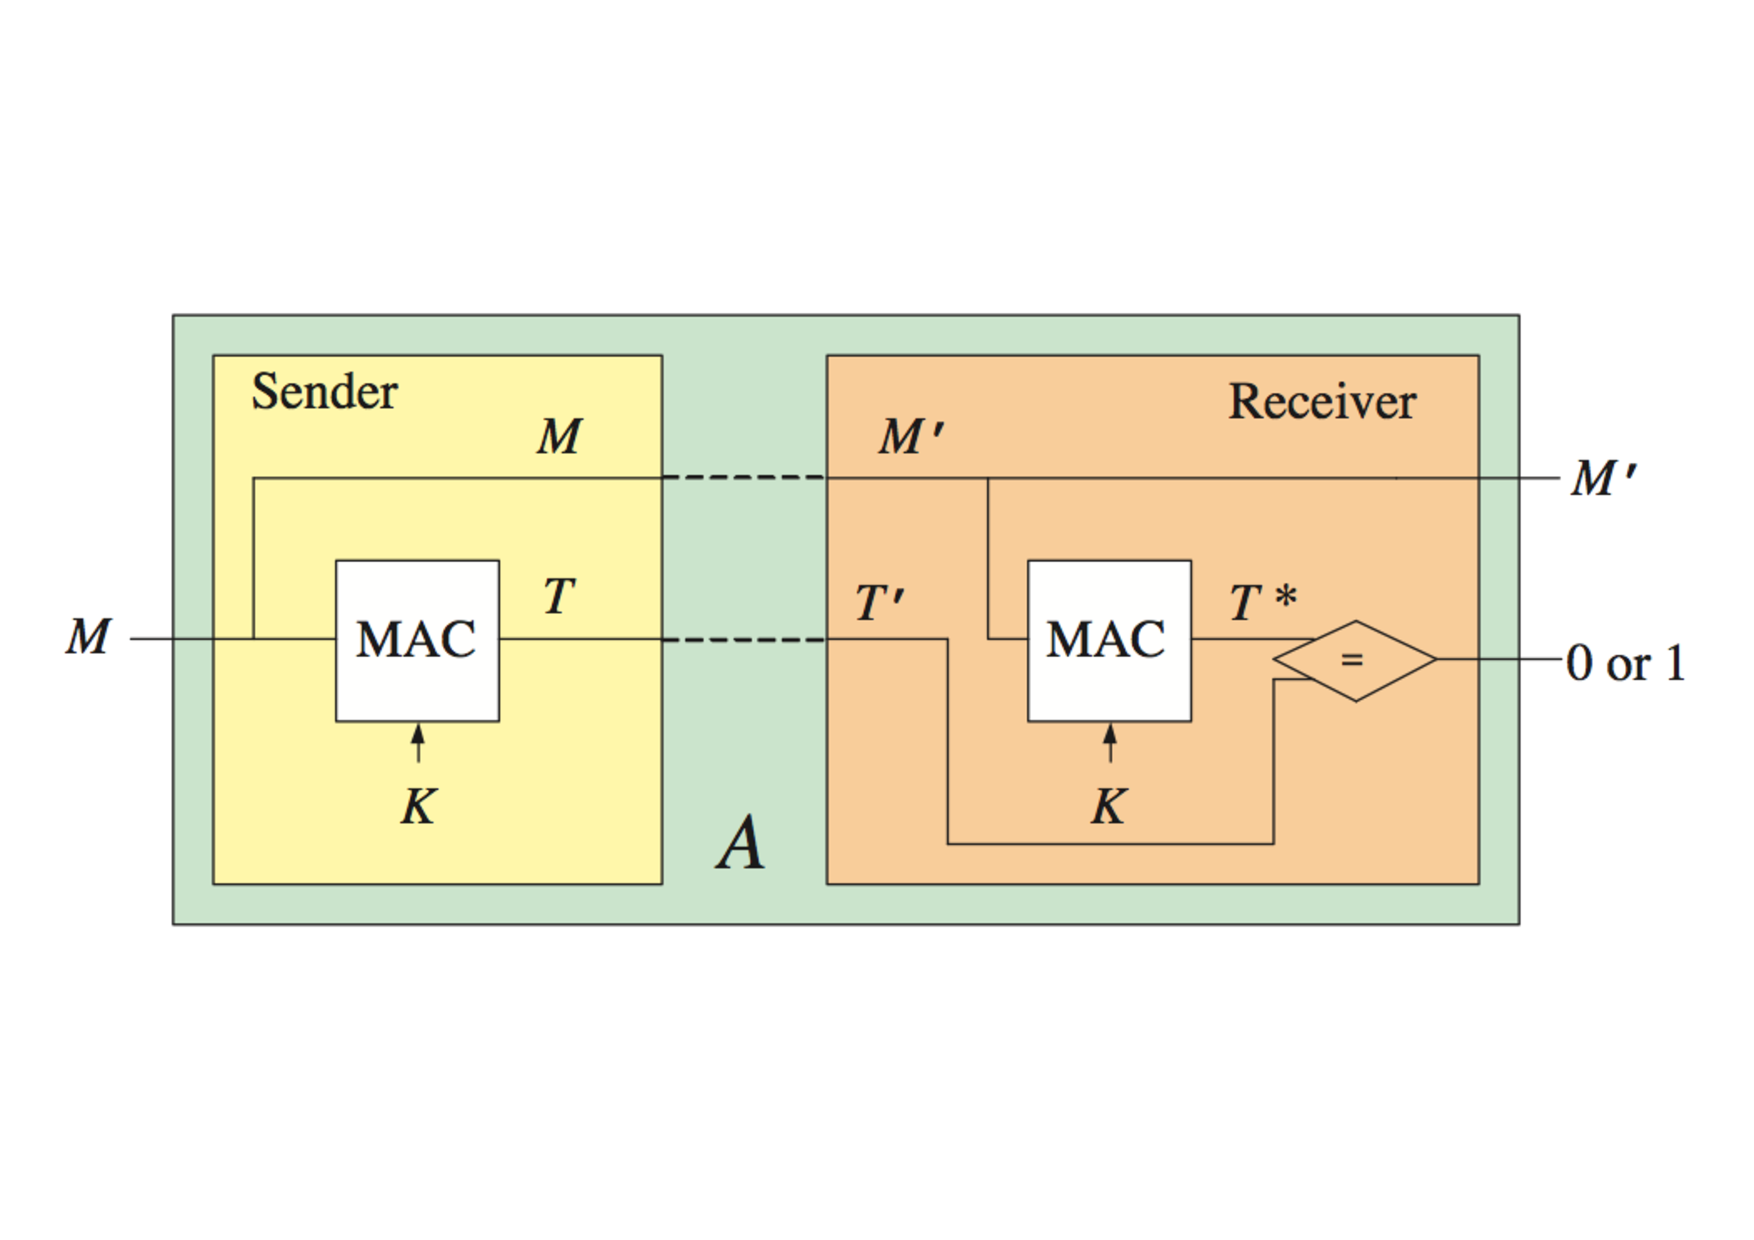
\includegraphics[scale=0.4]{./diagrams/MAC.pdf}
\caption{The Concept of Deterministic MAC Scheme}
\label{deterministic_mac }
\end{figure}
Message Authentication Code(MAC), called tag in some research works, is a short message block. A tag is generated by a MAC scheme by accepting a data block D as input and process D with a secret key K inside the scheme. Some MAC schemes require an additional input block, named nonce, in the generation of tag.  

When the processor writes a data block D to the memory, MAC scheme computes a tag  and concatenate the tag withe data forming a data-tag pair. The data-tag pair is sent to off-chip memory for storage.
When the processor reads a data from memory, the data-pair is sent to the chip and to MAC scheme. Assume the data part is D and tag part is T1. MAC scheme compute a tag T2 using D T2 is compared with T1. If T1 is identical to T2, D is assumed to be untampered.
 
Figure 3-b expresses the functionality of MAC scheme in integrity protection.

If the integrity of a processor-memory system is protected by MAC scheme, the possible attacks are:
\begin{enumerate}
	\item Modify the content of a data-tag pair
	\item Insert new data-tag pair
	\item Replace the content of a data-tag pair with a copy of data-tag pair from other address
	\item Replace the content of a data-tag pair with a copy of this pair in an old time point
\end{enumerate}
If a MAC scheme is capable to defend the 1st and 2nd attacks in the list, it should ensure that for any data block D, the tag is randomly assigned. If this scheme is capable to defend the 3rd and 4th attacks too, it should ensure for any two identical data blocks D1 and D2 that are writen to memory on different time or to different addresses, their tags T1 and T2 should be randomly generated.

\paragraph{Block-level  Added Redundancy Explicit Authentication (AREA)}
When the processor writes a data block D to memory, AREA concatenated a nonce N to D to form a data-nonce pair. This data-nonce pair is encrypted to form a ciphertext block E$_k$(D $\mid$ N). The ciphertext block is stored on off-chip memory.

When the processor reads a data block from memory, the ciphertext block is read to the chip and sent to AREA. After decryption, the nonce part of the pair, marked as N2, is compared to the nonce on-chip that is related to data D, marked as N1. If N1 and N2 are identical, D is assumed to be untampered.

If the integrity of a processor-memory system is protected by AREA, the possible attacks are:
\begin{enumerate}
	\item Modify the content of a E$_k$(D $\mid$ N)
	\item Insert new E$_k$(D $\mid$ N)
	\item Replace the content of a E$_k$(D $\mid$ N) with a copy from other address
	\item Replace the content of a E$_k$(D $\mid$ N) with a copy of this ciphertext block in an old time point
\end{enumerate}
If an AREA system is capable to defend the 1st and 2nd attacks in the list, it should ensure that for any data block D, the nonce is randomly assigned, which makes the cipherter block C=E$_k$(D $\mid$ N) a random value. If this scheme is capable to defend the 3rd and 4th attacks too, it should ensure for any two identical data blocks D1 and D2 that are writen to memory on different time or to different addresses, their nonces N1 and N2 should be randomly generated and make the related C1 and C2 random values.

\subsection{Security Evaluation for Authentication Primitives:the Approaches}
\subsubsection{Computational Provable Security}
\paragraph{The forgery attacks}
When attacking a message authentication system, the adversary try to send a pair(M,T) to the receiver to make VF$_k$(M,T)=1 while M did not originate with the legal sender. The fake pair(M$_f$,T$_f$) that makes VF$_k$(M$_f$,T$_f$)=1 is called a forgery from the adversary. A successful forgery attack indicates that the adversary has made a forgery. 
The purpose of a message authentication system is preventing the receiver to accept the message from unauthorized senders, such as an adversary. The quantitative property of a secure message authentication system is the low probability for an adversary to make a successful forgery attack with the limited resource.
\paragraph{Chosen-message attacks}
A strong type of attack that an adversary can conduct on the message authentication system is the adaptive chosen-message attack, marked as uf-cma. When doing uf-cma, the adversary chooses its own input message M and acquires the relative tag T. The adversary try to find the weakness in the design of message authentication system by analyzing the pairs(M,T) of his choice. The uf-cma provides the adversary with the most capability to succeed in the forgery attack. The probability that an adversary conducts a successful forgery attack after limited times of uf-cma is adopted as the basic quantitative security property of a message authentication in cryptography. This fact was also mentioned in \cite{Rogaway2011}.
\paragraph{The Security Notions of MAC schemes}
The formalised quantitative notion of the security of a MAC scheme was introduced by Bellare et al. in \cite{cbc1994}. This notion follows the security notion of digital signature introduced in \cite{signature}. The successful forgery on a MAC scheme from an adversary A is measured by a experiment called Forgery(MAC,A). In Forgery(MAC,A),  
the adversary A is provided a black-box access to the tag generation system TG$_K$(). When TG$_K$() takes an input message M$_i$, it returns tag T$_i$ to A. A conducts uf-cma by keep sending the message queries M$_i$ and observes the relative tag T$_i$ for limited times. On the other hand, A is provided a black-box access to the verification system VF$_K$(). When A sends a pair(M$_j$,T$_j$) to VF$_K$(), the VF$_K$() computes the tag T of M$_j$ and compares T with T$_j$. If T=T$_j$ then VF$_K$()=1 otherwise 0. If A sends a pair(M,T) that makes VF$_K$() outputs 1 while M has not appeared in the previous queries of uf-cma, then A succeeds a forgery attack and Forgery(MAC,A)=1.

The quantitative security notion of a MAC scheme is forgery probability, expressed as Forgery$_MAC$=Pr[Forgery(MAC,A)=1].
\paragraph{The Correlation between Security and Randomness}
Goldreich, Goldwasser, and Micali asserted in \cite{prf} that any good pseudorandom function(PRF) is a secure MAC scheme under the quantitative security notion. Bellare, Kilian and Rogaway proved this assertion in \cite{cbc1994} saying that if a system behave like a pseudoranom function, this system is a secure MAC scheme if meeting the requirements on domain and range of MAC schemes. Based on these two reduction of security notion, latter researches on security evaluation of MAC schemes posted their focuses on analyzing whether the MAC scheme evaluated behaves like a PRF.
\paragraph{The Randomness of a MAC scheme}
The definition of PRF was introduced in \cite{prf} indicating that PRF could not be distinguished from a ideal random function each bit of whose output was a coin flip. To define how closely a MAC scheme behaves like a PRF, Bellare et al. provided a quantitative notion in \cite{cbc1994} named Adv$^{PRF}_{MAC}$(), which was based on the concept of distinguisher introduced in\cite{prf}. 

Let F$_0$ and F$_1$ be two function with a common domain D and a common range R. A distinguisher A for F$_0$ versus F$_1$ is an adverary A that has access to a black box named oracle f:D->R. After accessing the oracle f, A computes a bit. Assume the function stored in the oracle f is X and A guesses that X is in the oracle, then A computes 1 otherwise 0. The the advantage of A in distinguishing F$_0$ from F$_1$ is expressed as Adv$^{F0}_{F1}$=Pr[f$\stackrel{R}{\longleftarrow}$F0:A$^{F0}$=1]-Pr[f$\stackrel{R}{\longleftarrow}$F1:A$^{F1}$=1]. Pr[f$\stackrel{R}{\longleftarrow}$F0:A$^{F0}$=1] means when the content of oracle f is F0, A guesses that F0 is in oracle then output 1.

We can see that if F0 behaves much like F1, it is hard for A to distinguish between F0 and F1 then Adv$^{F0}_{F1}$ is very small. This case is adopted by Bellare et al. in the quantitative notion of randomness of a MAC scheme. If the randomness of a MAC scheme is good, then the MAC scheme behaves like a PRF and Adv$^{[PRF]}_{MAC}$ is small. 

\subsubsection{Formal Method based Evaluation}
\subsubsection{Automated Sound Security Evaluation}


\subsection{Design Works of Authentication Primitives}
\paragraph{What to say in this subsection}
\begin{itemize}
	\item For each type of AP, the designs
	\item For each design, the security analysis and result
\end{itemize}

\subsubsection{Cryptographic Hash Functions}
Bellare, Canetti, and Krawczyk designed two authentication models in \cite{hmac}, the nested construction NMAC and the hash based scheme HMAC. The advantage of HMAC compared with MAC schemes constructed by block cipher is the fast processing speed and simpler in implementation. 
In this paper, the authors analyzed the security of NMAC and HAMC and provided a quantitative security result based on the security notion that HMAC is secure is the hash function used behaves like a PRF.  
\subsubsection{Message Authentication Code(MAC) Scheme}
\paragraph{Iterated MAC Schemes}
For a deterministic MAC scheme, a secrete key is used in processing message M and generating the tag T. The deterministic MAC design works can be categroized to iterated MAC scheme and parallel MAC scheme. 

In iterated MAC scheme, the process of a block in message M relys on the output of the process of its previous block. On the other hand, a block in message M can be processed only after its previous block finishes processing. 

\begin{figure}[htbp]
\centering
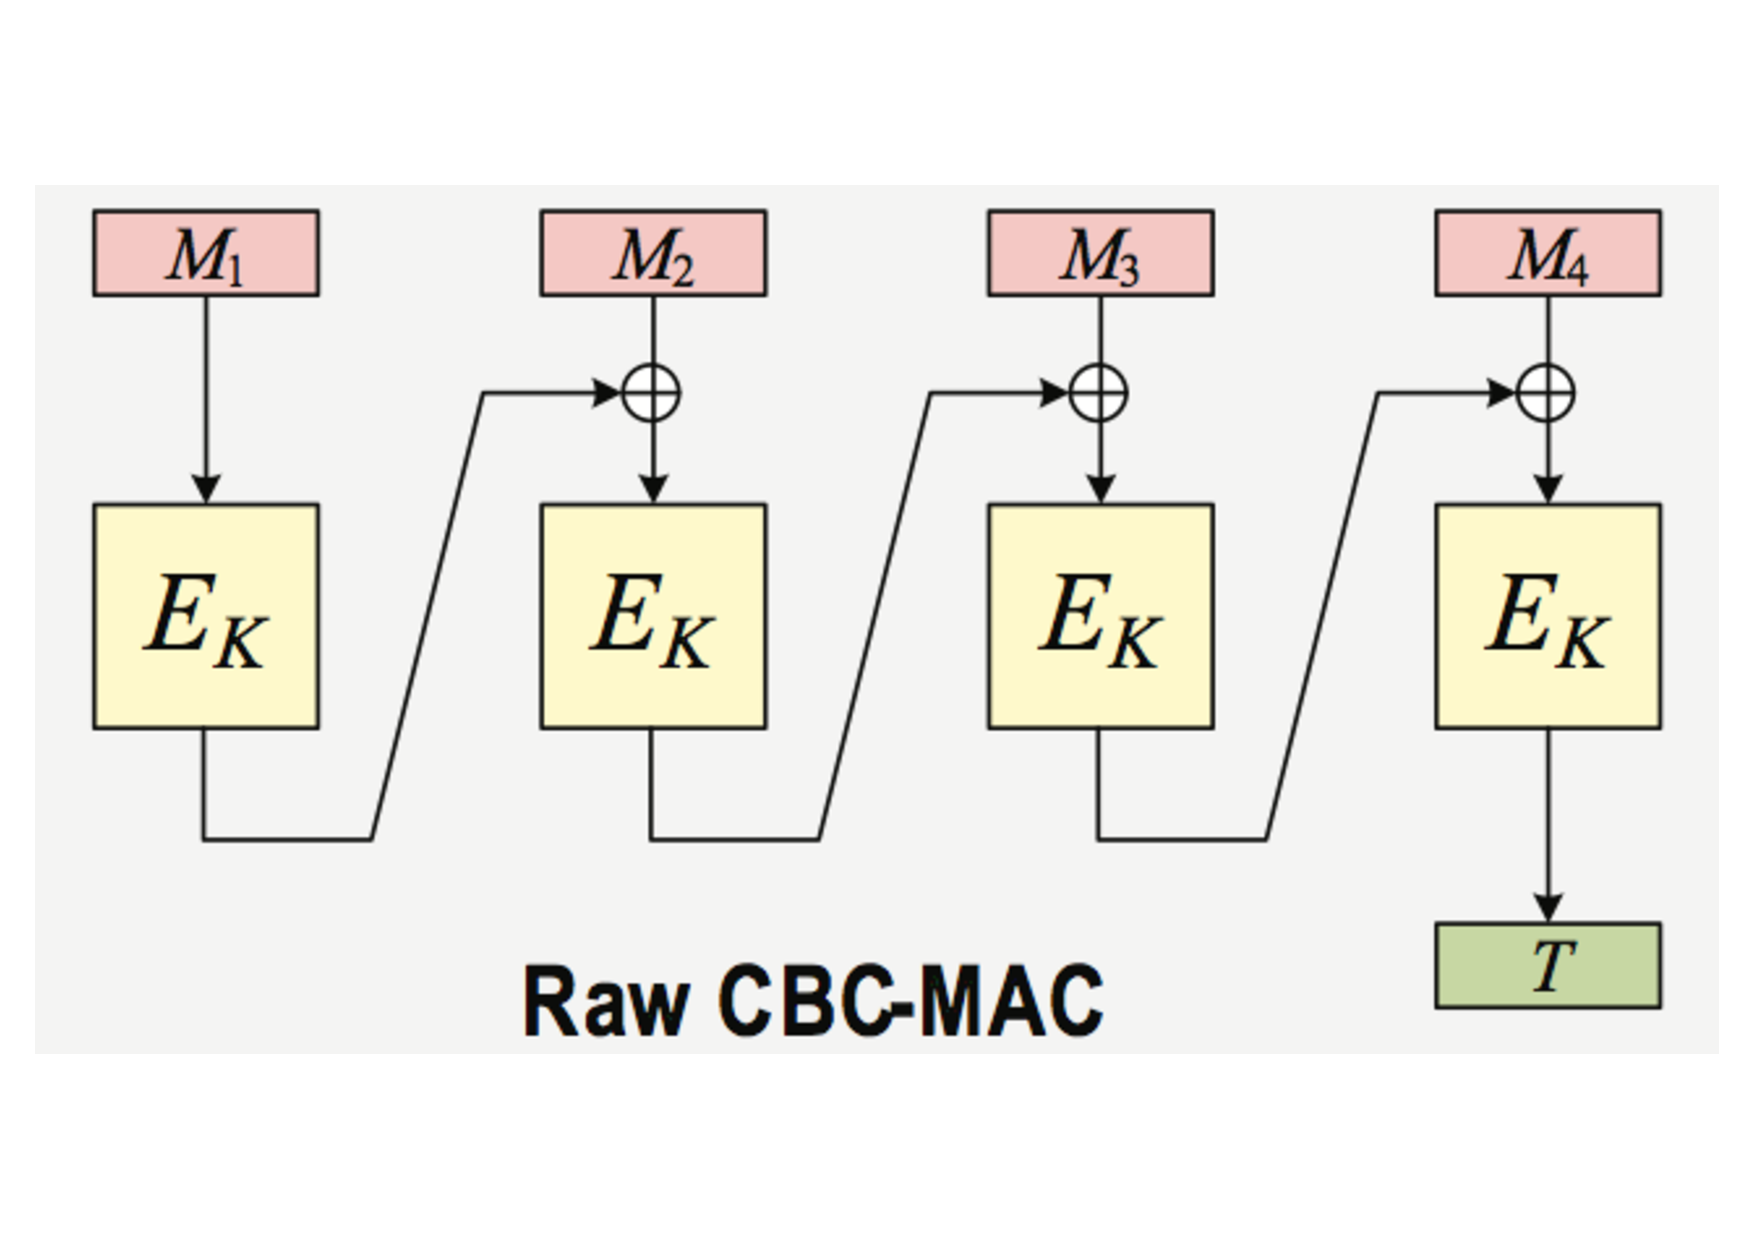
\includegraphics[scale=0.3]{./diagrams/cbc-mac.pdf}
\caption{The Raw CBC-MAC}
\label{CBC-mac }
\end{figure}
The research on iterated MAC schemes started from the raw CBC-MAC expressed in Figure 3.
\paragraph{Raw CBC-MAC}
The cryptographic primitive used in the raw CBC-MAC scheme is block cipher.  
The raw CBC-MAC is a secure MAC for only fixed length inputs. Assume the tag T of message M from CBC-MAC can be expressed as T = CBC-MAC$_k$(M), for another input M$\|$(M$\oplus$T), the tag T1=CBC-MAC(M$\|$(M$\oplus$T))=T. This attack indicates that the raw CBC-MAC is vulnerable if the input length is not fixed.
Besides the vulnerability when the input length is not fixed, the raw CBC-MAC scheme suffers birthday attack, means the adversary needs only 2$n/2$ input queries to succeed a forgery. 

Bellare et al. provided the original security evaluation on raw CBC-MAC\cite{cbc1994}. The conclusion is that if the adversary A is allowed to conduct arbitrary fixed length queries for q time, the probability that A succeeds in a forgery after the queries can be expressed with the queries times q and the computational assumption of block cipher used. Their quantitative conclusion showed that the forgery probability is very small.

\paragraph{EMAC}
The motivation of EMAC design is the problem that the raw CBC-MAC is secure only for fixed length inputs. 
EMAC is a optimized version of raw CBC-MAC providing security for arbitrary length inputs. The in the EMAC scheme, the final message block in the input is processed by a padding function to ensure that all the input blocks have the same length. Then raw CBC-MAC is applied applies and the result is encrypted by a the same block cipher in raw CBC-MAC with a different key. 

Petrank and Rackof provided the original security evaluation of EMAC in \cite{emac}. The EMAC is secure for arbitrary length inputs under the security notion if the block cipher meets the related computational assumptions. However, the EMAC still suffers the birthday attack.

\begin{figure}[htbp]
\centering
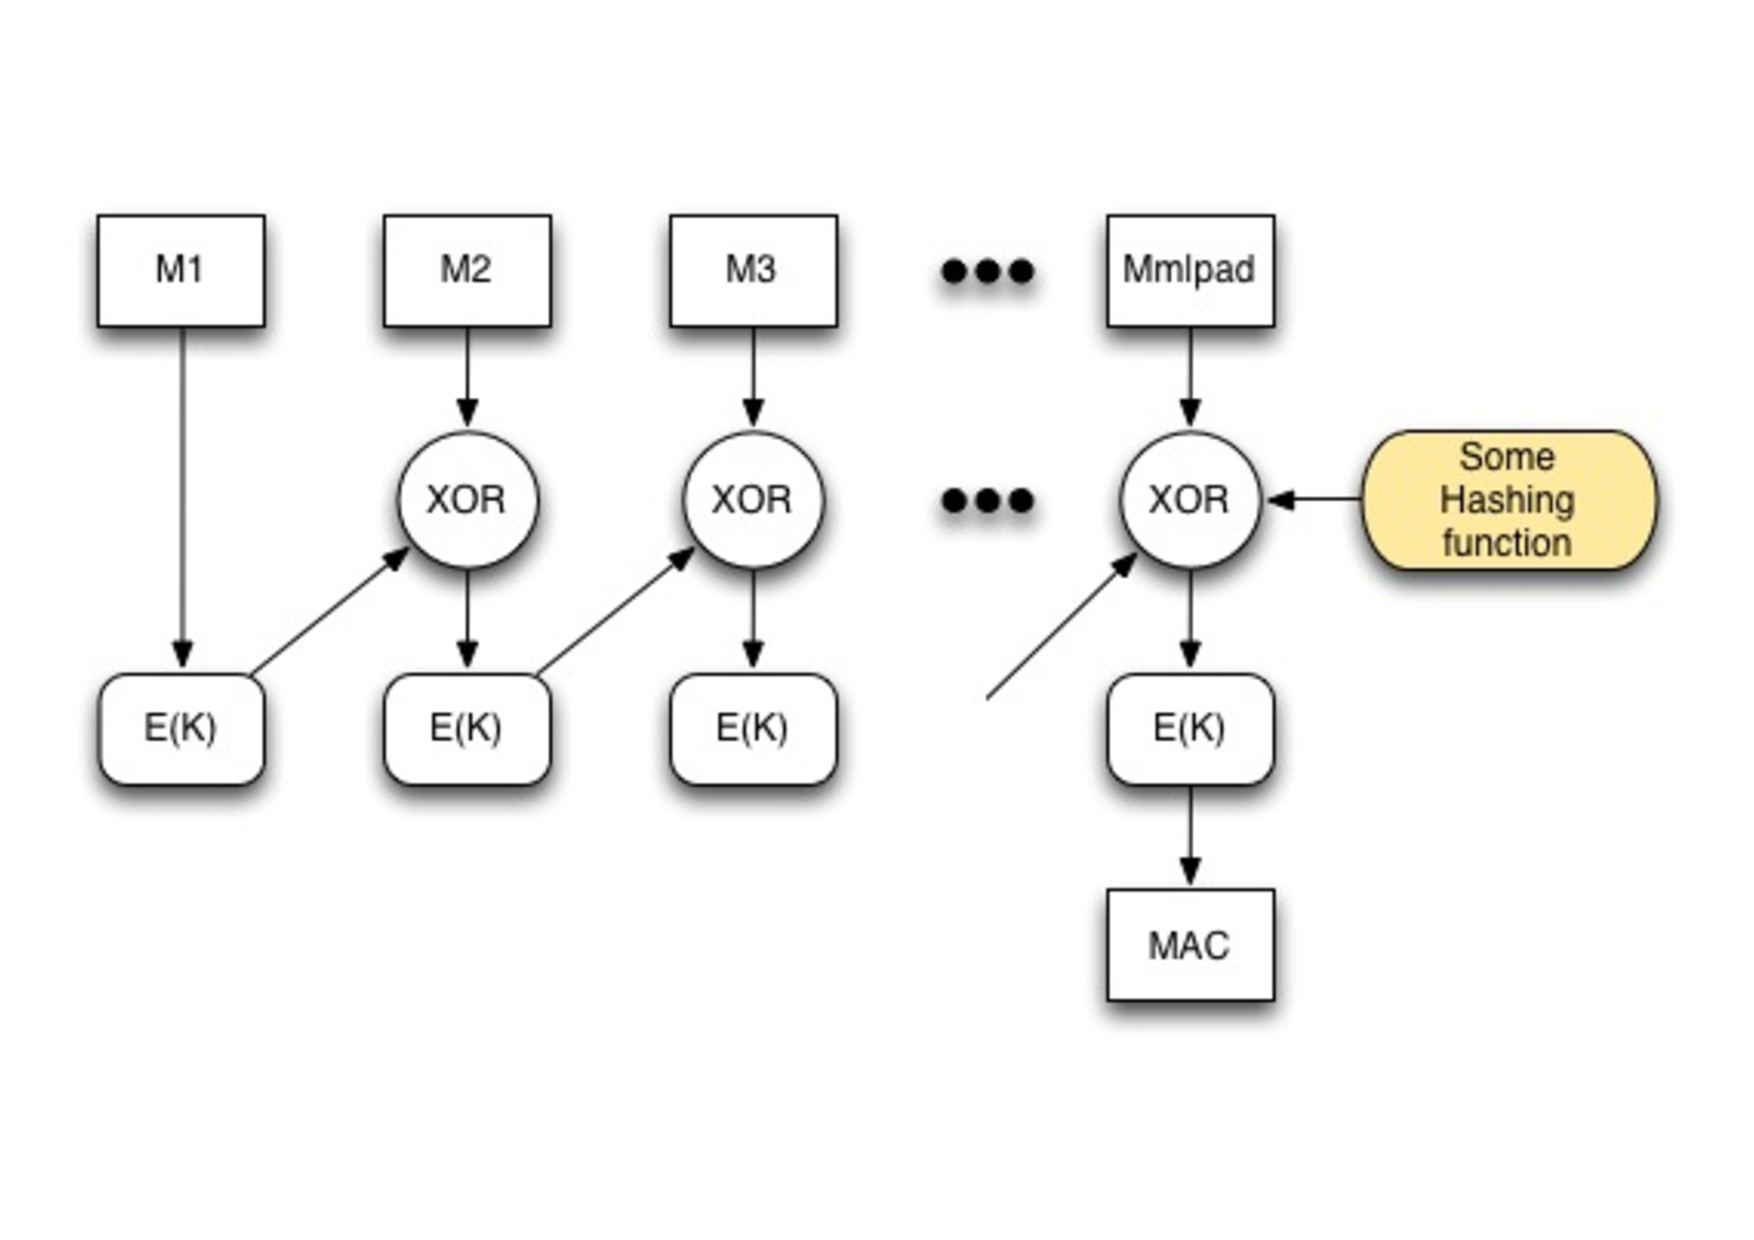
\includegraphics[scale=0.3]{./diagrams/cmac.pdf}
\caption{The class of CMAC}
\label{CMAC }
\end{figure}
Hence the raw CBC-MAC is vulnerable if the input length is not fixed, a class of MAC schemes named CMAC are developed to provide security for arbitrary length of inputs. The structure of the  variants of CMAC is modeled in Figure 4.
\paragraph{XCBC: three key version of CMAC }
Black and Rogaway introduced a optimized version of EMAC called XCBC in \cite{xcbc}.
There are two motivations of XCBC scheme: providing security for arbitrary length input; eliminate unnecessary padding operation on the input blocks in EMAC.

The XCBC scheme is a refined version of original EMAC. The contributions of XCBC scheme compared with the EMAC are: extending the domain to full domain; the block ciphers used in processing m input blocks is m other than m+1 in EMAC; all the block cipher in XCBC share a same key, the additional two keys are used to do exclusively or operation with the final input block,this design has faster processing speed.   

Black and Rogaway provided a original security analysis based on computational approach of XCBC scheme in \cite{xcbc}. Their quantitative result was improved by Minematsu and Matsushima in \cite{new}. 
Why the japanese want to optimize the original security bound? Any flaw in the proof? What is the advantage in the new proof procedure?
\paragraph{TMAC: two key version of CMAC}
Kurosawa and Iwata designed a optimized version of cmac requiring two different keys in \cite{tmac} named TMAC.  
The two different keys used in processing the final input blocks in XCBC are replaced by a keyed hash function with two distinct constants as inputs. This optimization aims to reduce the key cost. 

Kurosawa and Iwata provided an original security analysis on TMAC in \cite{tmac} showing that the same level of security was achieved by TMAC compared with XCBC. The original quantitative security conclusion of TMAC was improved by Minematsu and Matsushima in \cite{new}. 
\paragraph{OMAC: single key version of CMAC}
Iwata and Kurosawa introduced a optimization of original XCBC scheme with only one key, named OMAC in \cite{omac}. This key is used by the block cipher in the OMAC and the keyed hash function used in TMAC is replaced by a result of Galois field multiplication. OMAC is the variant of CMAC using the least number of keys. 

Iwata and Kurosawa provided an original security analysis on OMAC in \cite{omac}. This result have no optimized version yet.
\paragraph{other iterated MAC designs}
Daemen and Rijmen introduced a iterated MAC design named ALRED-MAC in \cite{alred}. The motivation of of this work is the limitation of quantitative security result for iterated MAC scheme due to the birthday paradox. 

\paragraph{Parallel MAC Schemes}
The motivation of designing MAC schemes in which input message blocks are processed in parallel is the latency of processing when using iterated MAC schemes. This latency becomes more obvious when run the scheme on processors supporting pipeline of parallelism. 
In parallel MAC scheme, all the blocks in message M are processed in parallel. The output blocks of M processing are transformed to a single block B, then processed to generate tag T. 
\paragraph{XOR MAC scheme}
Bellare, Guerin and Rogaway introduced a parallel MAC scheme named XOR MAC in \cite{xor-mac}. 
The parallel input processing makes the xor MAC faster the CBC-MAC. 
In \cite{xor-mac}, the authors provided a quantitative security conclusion of xor mac that it is security under the security notion of message authentication system if the pseudorandom function used in the design is secure. The security bound of xor mac from \cite{xor-mac} expressed a smaller result compared with the result of raw CBC-MAC. 

The main weakness of xor mac is the cost of storage for additional input parameters. According the design of xor mac, assume the input message is divided into m blocks and the length of each block is half of the length of block cipher input. Each input block has a index with domain as [1,m]. A input block is the concatenated with the encoder of its index(whose length is same as the input block) to form the input to a block cipher, for example (i$\|$M[i]). Besides the m concatenated input blocks, a nonce formed with random number or counter is used a input to the block cipher. Then the m+1 output blocks from block cipher is xored and the output block of xor operation is concatenated with a random number or counter to form the final tag. 
We can see that the length of tag from xor-mac is the sum of the length of a output block from block cipher and the length of a random number or counter. This long-length MAC needs additional storage compared with the tag from iterated MAC schemes. 
On the other hand, the nonce maintained by the user of xor mac is regarded a disadvantage by some researchers.

\paragraph{Raw PMAC}
Black and Rogaway introduced an parallel MAC scheme named PMAC in \cite{pmac}. 
The improvement of PMAC compared with XOR MAC is the less calling of block cipher when generating a tag. Secondly, there is no limitation for the input length when using PMAC. 
Another benefit brought by PMAC is that only one key is needed in generating the tag. Other processing operations include bit-level xor and gray code, which are cost-effective and fast processing. 

The quantitative security result of PMAC was acquired by Black and Rogaway in \cite{pmac}. They analysed the probability of internal collision in the arbitrary types of inputs and asserted that the PMAC design is a secure MAC if the block cipher used behaves like a pseudorandom permutation. In the proof from Black and Rogaway, the probability that an adversary can distinguish the PMAC from pseudorandom function is the probability that collsion of internal blocks(the outputs of block cipher) plus the probability of tag collision. 

Lee et al. posted attacks on the raw PMAC in \cite{pmac_forgery}. Their research indicated that the raw PMAC design did not bring advantage in security compared with iterated MACs. The raw PMAC suffers from their birthday like attack and the key recover attack.
 
\paragraph{Tweakable block cipher and Optimized PMAC}
The concept of tweakable block cipher was formally defined by Liskov, Rivest, and Wagner in \cite{tweak}. Rogaway introduced a efficient implementation of tweakable block cipher in \cite{tweak_pmac}and adopt this implementation to replace the block cipher used in the original PMAC and OCB authenticated encryption mode.
The application of tweakable block cipher in constructing PMAC can enhance the processing speed compared with original PMAC based on Grey code and simplify the structure of the scheme, which also simplifys the security analysis of the scheme . 

In \cite{tweak_pmac}, Rogaway provided an assertion that the tweakable block cipher XE and XEX behave like a pseudorandom permutation if the block cipher inside is a pseudorandom permutation. Based on this assertion about security of tweakable block cipher, Rogaway gave an quantitative conclusion that the new PMAC based on tweakable block cipher is security under the security notion of message authentication system. This quantitative security result of tweakable block cipher based PMAC was provided in \cite{tweak_pmac}.
Minematsu and Matsushima optimzed this result in \cite{new}. 

The evaluation procedure in \cite{pmac} is questioned by the latter researchers hence the correlation between collision probabilty and 
distinguishing probability was not explained . This issue was also pointed in Nandi`s improved analysis on PMAC in \cite{improve_pmac}. Nandi also provided a improved quantitative security result of PMAC which is smaller in all the cases than the one in \cite{pmac} and \cite{new}. 

\paragraph{iPMAC}
Sarkar introduce an optimisation on original PMAC in \cite{iPMAC}. The galois field multiplication used in the tweakable block cipher introduced is replaced by a technique named tower field representation of Galois field. This replacement enhance the processing speed in software.

Hence the structure of iPMAC is same as the original PMAC except the input masking stage, the security evaluation by the author in \cite{iPMAC} followed the approach in \cite{pmac}.

\paragraph{Stately MAC Schemes}
Deterministic MAC schemes cannot defend against the second type of attack in the threat model defined in Section 1.1.1 . The reason is that the secrete key used in genrating the tag will not be refreshed for each message. If two message are identical, their tags are identical. To address this issue, nonce is introduced to the tag generation in a MAC scheme. A nonce is a short message block whose value will be updated by each message in tag generation. To update the value of nonce, the address of message, a random number, a counter or the combination of these three elements are adopted in the nonce generation for each message. With the nonce introduced, a well designed stately MAC scheme should be capable in defending type 2 attack in threat model.
\paragraph{GMAC and GCM}
McGrew and Viega introduced the Galois/Counter Mode authenticated encryption design and the original security analysis is provided in \cite{gcm}. The message authentication system in GCM(named GMAC) is a iterated scheme based on the concept of universal hashing. The block processing component used in GMAC is the Galois field multiplication other than the block cipher in deterministic MAC schemes. 
The motivation of GCM is to design a scheme combining counter mode of operation(CTR) with a message authentication code(the GMAC) to form a efficient and secure authenticated encryption system.
One advantage of adopting the Galois field multiplication in GMAC is that it can be made easily in hardware and has efficient performance in software. 

In the security analysis of GCM from McGrew and Viega, the GMAC was not discussed alone. The security of GMAC as a message authentication code is based on the fact that the encryption part in GCM is secure and the collision probability of ciphertext blocks is low. 
In GCM design, the nonce is called initialization vector (IV). For each invocation of GCM, the IV should be distinct.

In \cite{breaking}, Iwata, Ohashi and Minematsu provided an optimised analysis for the security of GCM. They pointed out the weakness in the lemma used in forming the bound of the quantitative result of security for GCM with a counter example. This counter example was developed to a distinguishing attack on GCM. Iwata et al. then provided a approach fixing the problem of original lemma and provided the new quantitative security result of GCM. 

In \cite{Rogaway2011}, Rogaway pointed the weakness of GMAC as a MAC scheme when used alone that the security under adaptive chosen-message attack is not as good as the security of deterministic MAC schemes. On the other hand, GMAC requires the nonce for tag generation and this nonce should be maintained and refreshed by the user of GMAC. The potential issue of this design pointed by Rogaway is the reuse of nonce, which may lead to the collision of the tag. 

Handschuh and Preneel introduced key-recovery attacks on universal hash function based MAC algorithms in \cite{key_recover}. They introduced two types of attacks: weak key finding and partial information leaks.

\paragraph{Cost-Effective Tag Design}
Hong, Guo and Hu introduced a parallel MAC design in \cite{cetd}.
In their design, the inputs are ciphertext blocks(called encrypted cache line in this paper). A nonce is generated by encrypting a (address,counter,random) pair and then used in controlling the tag generation. The pair used in generating the nonce is consist of the virtual address of the ciphertext blocks, a random number and a counter. The inputs are processed in two stages: bit segment swap between 2 input blocks for several rounds and the block rotate shift. The parameters of each stage are segements in the nonce.

\subsubsection{The Authenticated Encryption Schemes}
After various kind of MAC schemes were evaluated and claimed to be secure, a new cryptosystem, the Authenticated Encryption(AE) was introduced The Authenticated to combine the encryption of
plaintext blocks and generation of the MAC in a single scheme to provide both
confidentiality and integrity. The methodology of constructing a AE scheme was categorized by
Bellare in \cite{AE_mode}. In this paper, the author claimed that according to
the 3 types of modes defined, the most secure one was the Encrypt-then-MAC mode.
In Rogawa`s works \cite{aead} a systematical analysis about AE
schemes using associate data was expressed.  

Based the notion of security evaluation for AE systems introduced in \cite{aead}, the security of several AE schemes in
Encrypt-then-MAC mode have been analyzed systematically, including CCM \cite{ccm}based on
CBC-MAC,EAX\cite{eax} based on OMAC, GCM
\cite{gcm} based on universal hashing(new bound revised in \cite{breaking}), and
OCB\cite{ocb} based on PMAC(new bound revised in \cite{tweak,iPMAC}). Kasper and
Schwabe introduced a implementation of AES that run faster than previous AES block cipher
and adopted this implementation to construct a faster AES-GCM AE
scheme\cite{fast}.

There were research works on attacks to existing authentication system or AE systems, such as
\cite{cycle,attack_blk,hardware_attack}. Some of these works recover the security weakness in the design works while some other works depict attacks that are out of the security bound of system analyzed. 


\subsubsection{Block-level Added Redundancy Explicit Authentication (AREA)}

\subsection{Message Authentication(MA) Systems:: the Implementation of Theoretical Model}
\paragraph{What to say in this subsection}
\begin{itemize}
	\item The MA system design
	\item For each MA system, the security analysis and result
\end{itemize}

\paragraph{Concepts of Message Authentication(MA) System}
After the Authentication Primitives are evaluated systematically, researchers have paid effort on designing message authentication system on-chip based on these primitives.
In the design of on-chip message authentication system, the on-chip data is assumed to be inaccessible and secure, and the chip is called trusted area; while the data in the transmission and stored in off-chip memory is considered to be accessible to attackers and vulnerable. Transmission path(such as bus) and off-chip memory are called malicious area. 
\begin{figure}[htbp]
\centering
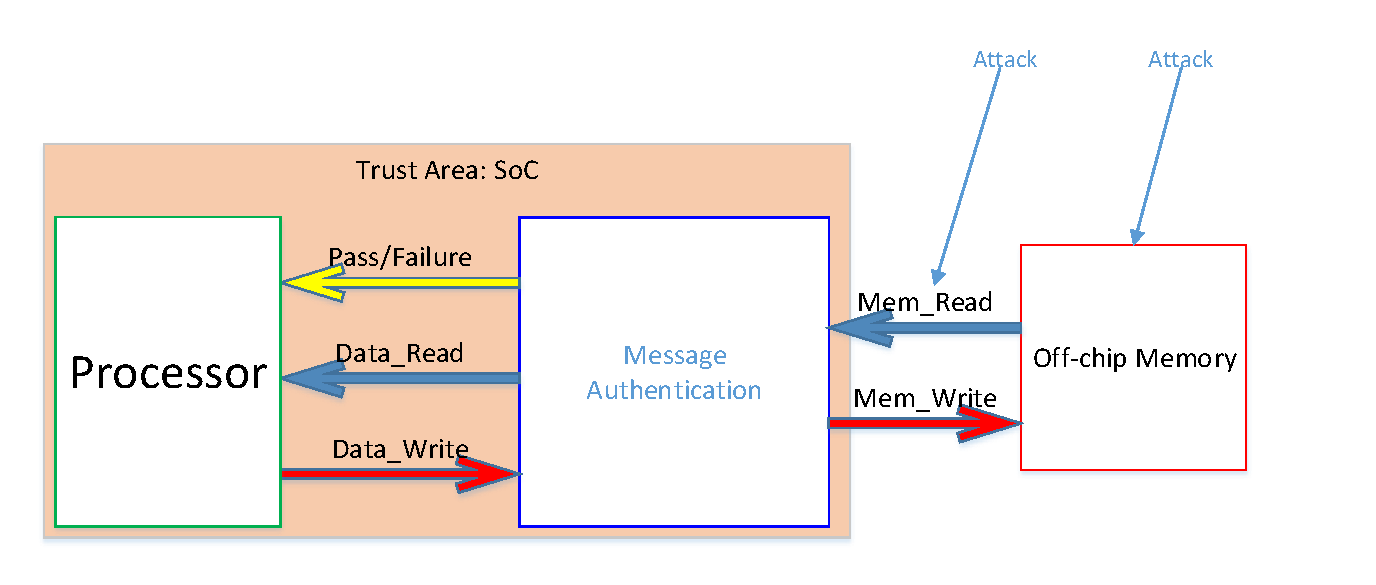
\includegraphics[scale=0.5]{./diagrams/MA_concept.pdf}
\caption{The Concept of MA System}
\label{ma_system}
\end{figure}

Figure 1 expresses the concept of MA system for processor-memory communication. 
When processor writes a data block, marked as D, to and address, marked as addr, on the memory, processor sends D to MA system and output a message block, marked as message(D, add$_B$), where add$_B$ represents an additional data block. The message block message(D,add$_B$) can be the data block D only, D concatenated with a short block(commonly called tag) or other format of D. The content of message(D,add$_B$) is determined by the crypographic primitive adopted by the MA system.
When the processor wants to read the data D from address addr, the message(D,add$_B$) is read to SoC and sent to MA system first. After verified by MA, if the data D is not tampered, MA sends a signal indicating pass to processor and send the D to the processor, where D is extracted from message(D,add$_B$) block read from memory.
If the MA system finds that the D is tampered, MA sends a failure signal to processor, and invoke the exception handling procedure.
\paragraph{Security Evaluation for MA Systems}


\subsubsection{Hash Function Based MA Systems}
\paragraph{Uniprocessor System}
In 2003 \cite{keylist}, Suh et al. introduced a hardware design aiming to provide protection the confidentiality and integrity of off-chi memory. In their design, the message authentication system is based on a hash function.

Gassend et al. developed a integrity verification mechanism in 2003 \cite{keylist}. Merkly tree, AP is hash function or MAC.

  


\paragraph{Multiprocessor System}


\subsubsection{MAC Function Based MA Systems}
\paragraph{Uniprocessor System}
XOM: vulnerable to replay attack, analyzed by another paper

Yan`s design: 
\begin{itemize}
	\item the AP is GCM, faster than hash(MD5)
	\item timely authentication
	\item What add data is stored on-chip? what is stored off-chip on memory? On-chip cost?
	\item How to ensure the IV distinct?
\end{itemize}use timely authentication other than lazy authentication. use fast authentiation method other than hash(MD5).

Rogers` design:protect code and data; 
Mei`s design:
\paragraph{Multiprocessor System}

Shi et al. proposed a MA system for multiprocessor shared memory architecture. It is an Encrypt-and-MAC scheme and the MAC is generated with hash function Sha 256.
\subsubsection{Block-level AREA Based MA Systems}
\paragraph{Uniprocessor System}
\paragraph{Multiprocessor System}

\bibliographystyle{plain}
\bibliography{./resources/tag_paper.bib}
\end{document}